\item \textbf{{[}ALVL/9597/2017/P2/Q6{]} }

A computer company has several offices throughout the country, each
with several salespersons. A record of the sales made by each salesperson
has been set up using a relational database. There is a minimum amount
of \$150 for each sale.

The following tables hold the data. 

\texttt{CUSTOMER (}\texttt{\uline{CustomerID}}\texttt{, CustomerName,
CustomerEmail, CustomerTelephone) }

\texttt{OFFICE (}\texttt{\uline{OfficeID}}\texttt{, Address, Telephone) }

\texttt{SALE (}\texttt{\uline{CustomerID{*}}}\texttt{, }\texttt{\uline{SalesPersonID{*}}}\texttt{,
SaleDate, Amount) }

\texttt{SALESPERSON (}\texttt{\uline{SalesPersonID}}\texttt{, SalespersonName,
OfficeID{*}) }

\textbf{Note:} underline indicates primary key. An asterisk ({*})
indicates a foreign key. 
\begin{enumerate}
\item Draw an Entity-Relationship (E-Fl) diagram to represent the data model.
\hfill{} {[}3{]} 
\item (b) The following is a section of the data dictionary for the data
model. it has three missing entries labelled \textbf{A}, \textbf{B
}and \textbf{C}.
\begin{center}
\begin{tabular}{|l|l|l|c|}
\hline 
\texttt{\textbf{\hspace{0.01\columnwidth}}}\textbf{Table} & \texttt{\textbf{\hspace{0.01\columnwidth}}}\textbf{Field} & \textbf{Data type} & \textbf{Validation}\tabularnewline
\hline 
\texttt{CUSTOMER} & \texttt{CustomerID} & Integer & Unique\tabularnewline
\hline 
\texttt{SALE} & \texttt{CustomerID} & Integer & \textbf{A}\tabularnewline
\hline 
\texttt{SALE} & \texttt{SaleData} & Date & \tabularnewline
\hline 
\texttt{SALE} & \texttt{Amount} & \texttt{\textbf{\hspace{0.01\columnwidth}}}\textbf{B} & \textbf{C}\tabularnewline
\hline 
\end{tabular}
\par\end{center}

State a suitable entry for \textbf{A}, \textbf{B} and \textbf{C}.
\hfill{}{[}3{]} 
\item There is an address field in this database.

Explain why storing the address as a single field is not good database
design. \hfill{}{[}3{]}
\end{enumerate}
Each month, a report is produced to show the sales for each salesperson.
The following is a report for salesperson, B Chin. 
\begin{center}
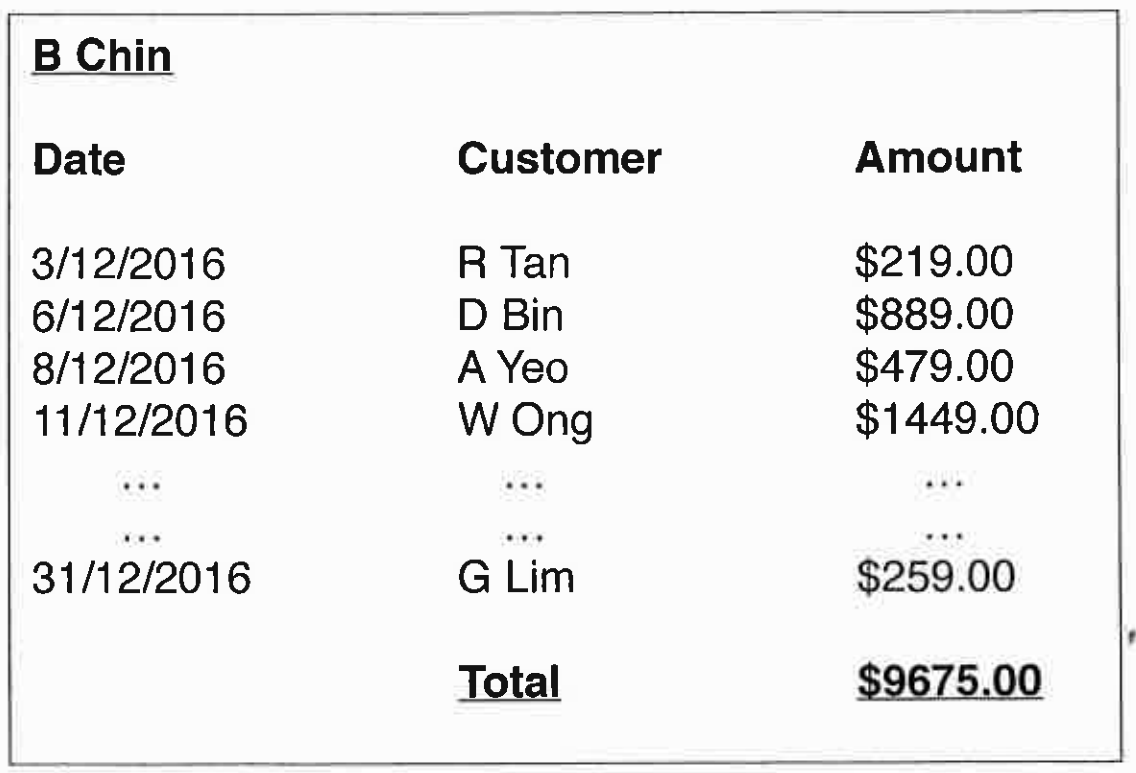
\includegraphics[width=0.5\paperwidth]{C:/Users/Admin/Desktop/Github/question_bank/LyX/static/img/9597-ALVL-2017-P2-Q6}
\par\end{center}
\begin{enumerate}
\item[(d)] {}
\begin{enumerate}
\item To produce the report, the database uses the \texttt{SaleDate} and
\texttt{Amount} fields in the \texttt{SALE} table. 

Name \textbf{four }other fields that the database uses to produce
this report.\hfill{} {[}4{]}
\item State \textbf{two} features of a relational database management system
which would be used to calculate and display the total for this salesperson.\hfill{}
{[}2{]}
\end{enumerate}
\end{enumerate}